\section{EC2 Section}

\subsection{Amazon EC2}

\begin{itemize}
	\item EC2 is one of the most popular of AWS's offering (EC2 là một trong những sản phẩm nổi tiếng nhất được cung cấp bởi AWS)
	\item EC2 = Elastic Compute Cloud = Infrastructure as a Service
	\item It mainly consists in the capability of:(Nó chủ yếu nằm ở khả năng của:)
	\begin{itemize}
		\item Renting virtual machines (EC2)
		\item Sorting data on virtual drives (Sắp xếp dữ liệu trên ổ đĩa ảo)(EBS)
		\item Distributing load across machines(chia tải công việc ra giữa nhiều máy khác nhau) (ELB)
		\item Scaling the services using an auto-scaling group (Mở rộng dịch vụ bằng cách sử dụng nhóm tự động mở rộng) (ASG)
	\end{itemize}
	\item Knowing  EC2 is fundamental to understand how the Cloud works
\end{itemize}

\subsection{EC2 sizing \& configuration options}

\begin{itemize}
	\item Operating System (OS): Linux, Windows or Mac OS
	\item How much compute power \& cores 
	\item How much random-access memory
	\item How much storage space:
	\begin{itemize}
		\item Network-attached
		\item hardware (EC2 Instance Store)
	\end{itemize}
	\item Network card:  speed of the card, public IP address
	\item Firewall rules:security group
	\item Bootstrap script(configure at first launch): EC2 User Data
\end{itemize}

\subsection{EC2 User Data}


\begin{itemize}
	\item It is possible to bootstrap our instances using an EC2 User Data script
	\item bootstrapping means launching commands when a machine start
	\item That script is only run once at the instance first start 
	\item EC2 user data is used to automate boot tasks such as: 
	\begin{itemize}
		\item Installing updates
		\item Installing software
		\item Downloading common files from the internet
		\item Any thing you can think of
	\end{itemize}
	\item The EC2 User Data Script runs with the root user
\end{itemize}


\subsection{EC2 Instance Types - Overview}

\begin{itemize}
	\item You can use different types of EC2 instances that are optimised  for different use cases
	\item AWS has following naming convention:
	\begin{center}
		m5.2xlarge
	\end{center} 
	\item m: instance class
	\item 5:generation (AWS improves over time)
	\item 2xlarge: size within instance class
\end{itemize}


\subsection{EC2 Instance Types - General Purpose}

\begin{itemize}
	\item Great for a diversity workloads such as web servers or code repositories (Tuyệt vời cho nhiều khối lượng công việc khác nhau như máy chủ web hoặc kho lưu trữ mã)
	\item Balance between:
	\begin{itemize}
		\item Compute
		\item Memory
		\item Network
	\end{itemize}
\end{itemize}

\subsection{EC2 Instance Types - Compute Optimized}

\begin{itemize}
\item Great for compute-intensive tasks that require high-performance processors: \\ 
(Rất tuyệt cho các nhiệm vụ tính toán chuyên sâu yêu cầu bộ xử lý hiệu năng cao)
\begin{itemize}
	\item Batch processing workloads \\ Xử lý khối lượng công việc theo từng đợt
	\item Media transcoding \\ Chuyển đổi định dạng phương tiện 
	\item High-performance web servers \\ Các máy chủ web hiệu năng cao
	\item High-performance computing (HPC) \\ Tính toán hiệu năng cao
	\item Scientific modeling \& machine learning \\ Mô hình hóa khoa học và học máy
	\item Dedicated gaming servers \\ Máy chủ trò chơi chuyên dụng
\end{itemize}
\end{itemize}

\subsection{EC2 Instance Types - Memory Optimized}

\begin{itemize}
	\item Fast performance for workloads that process large datasets in memory \\
	Hiệu năng nhanh chóng cho các tác vụ xử lý bộ dữ liệu lớn trong bộ nhớ
	\item Use cases:
	\begin{itemize}
		\item High performance, relational/non-relational databases 
		\item Distributed web-scale cache stores \\ Các kho bộ nhớ đệm phân tán ở quy mô web
		\item In-memory databases optimized for BI (business intelligent) Các cơ sở dữ liệu trong bộ nhớ được tối ưu cho BI
		\item Applications performing real-time processing of big unstructured data \\ Các ứng dụng thực hiện xử lý trong thời gian thực với dữ liệu lớn không có cấu trúc
	\end{itemize}
\end{itemize}


\subsection{EC2 Instance Types - Storage Optimized}
\begin{itemize}
	\item Great for storage-intensive tasks that require high, sequential read and write access to large datasets on local storage \\
	Tuyệt vời cho các tác vụ yêu cầu lưu trữ cao, với khả năng đọc/ghi tuần tự hiệu suất cao trên các bộ dữ liệu lớn được lưu trữ cục bộ
	\item Use cases:
	\begin{itemize}
		\item High frequency online transaction processing (OLTP) systems \\ Hệ thống xử lý giao dịch trực tuyến (OLTP) với tần xuất cao
		\item Relational \& NoSQL databases
		\item Cache for in-memory databases (for example, Redis) \\Bộ nhớ đệm cho các cơ sở dữ liệu trong bộ nhớ (ví dụ: Redis)
		\item Data warehousing applications \\ Các ứng dụng kho dữ liệu
		\item Distributed file systems
	\end{itemize}
\end{itemize}


\subsection{Introduction to Security Groups}

\begin{itemize}
	\item Security Groups are fundamental of network security in AWS
	\item They control how traffic is allowed into or out of our EC2 Instances 
	\item Security groups only contain allow rules
	\item Security groups rules can reference by IP or by security group
\end{itemize}


\begin{figure}[htbp]
	\centering
	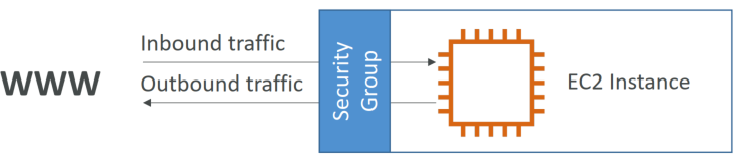
\includegraphics[width=1\linewidth]{images/security-groups-traffic.png}
	\caption{security-groups-traffic}
	\label{fig:security-groups-traffic}
\end{figure}

\subsection{Security Groups - Deeper Dive}
\begin{enumerate}
	\item Security groups are acting as a "firewall" on EC2 Instances
	\item They regulate:
	\begin{itemize}
		\item Access to Ports
		\item Authorised IP ranges - IPv4 and IPv6
		\item Control of inbound network (from other to the instance) \\ Kiểm soát các kết nối bên ngoài đi vào bên trong hệ thống
		\item Control of outbound network (from the instance to other) \\ Kiểm soát các kết nối từ bên trong hệ thống đi ra bên ngoài
	\end{itemize}
\end{enumerate}

\subsection{Security Groups - Diagram}

\begin{figure}[htbp]
	\centering
	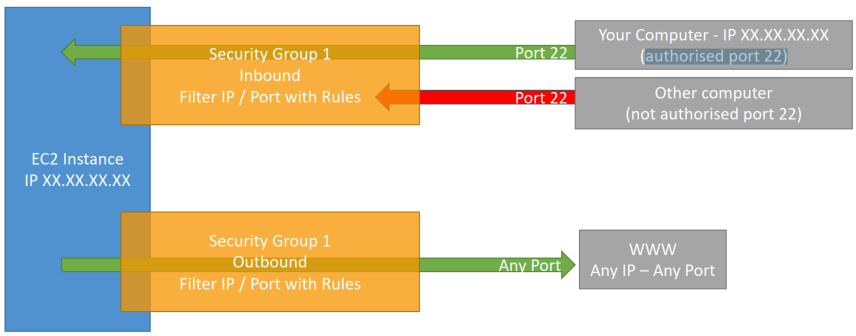
\includegraphics[width=1\linewidth]{images/security-groups-diagram.png}
	\caption{security-groups-diagram}
	\label{fig:security-groups-diagram}
\end{figure}

\subsection{Security Groups - Good to know}

\begin{itemize}
	\item Can be attached to multiple instances
	\item Locked down to a region / VPC combination (Bị giới hạn hoặc ràng buộc trong một cặp region và vpc cụ thể)
	\item Does live "outside" the EC2 - if traffic is blocked the EC2 instance won't see it
	\item It's good to maintain one separate security group for SSH access (Việc tách riêng các security groups cho ssh là điều nên làm)
	\item If your application is not accessible (timeout), then it's a security group issue
	\item If your application gives a "connection refused" error, then it's an application error or it's not launched
	\item All inbound traffic is blocked default
	\item All outbound traffic is authorised by default
\end{itemize}



\subsection{Referencing other security groups - Diagram}

\begin{figure}[htbp]
	\centering
	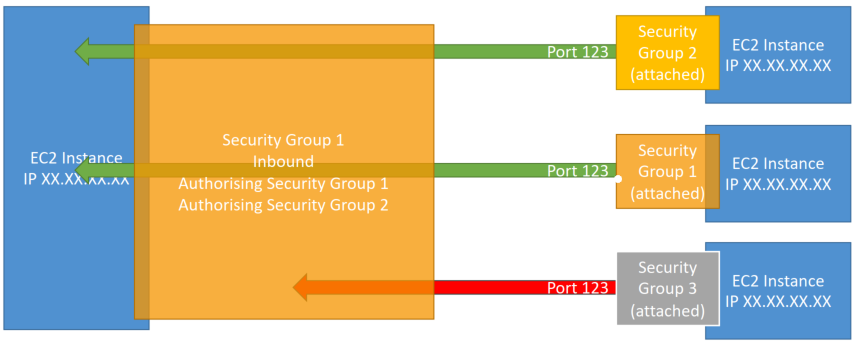
\includegraphics[width=1\linewidth]{images/referencing other security groups - diagram.png}
	\caption{referencing other security groups - diagram}
	\label{fig:referencing other security groups - diagram}
\end{figure}

\subsection{Classic Ports to know}

\begin{itemize}
	\item 22 = SSH (Secure Shell) - log into a Linux instance
	\item 21 = FTP (File Transfer Protocol) - update files into a file share
	\item 22 = SFTP (Secure File Transfer Protocol) - upload files using SSH
	\item 80 = HTTP - access unsecured websites
	\item 443 = HTTPS - access secured websites
	\item 3389 = RDP (Remote Desktop Protocol) - log into a Windows instance
\end{itemize}

\newpage

\subsection{SSH Summary Table}

\begin{figure}[h]
	\centering
	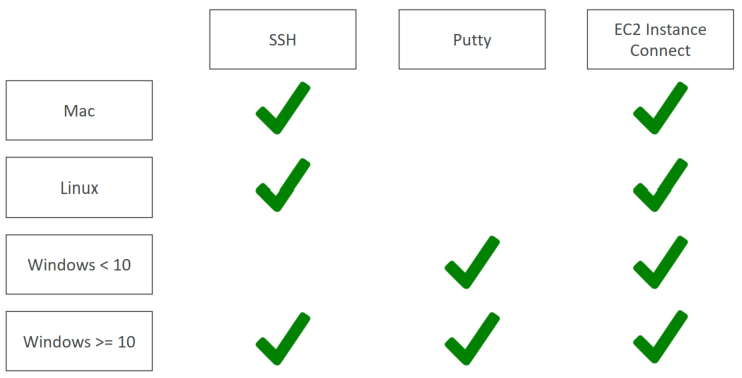
\includegraphics[width=1\linewidth]{images/ssh-summary-table.png}
	\caption{ssh-summary-table}
	\label{fig:ssh-summary-table}
\end{figure}



\subsection{How to SSH into your EC2 Instance -  Linux/Mac OS X}

\begin{itemize}
	\item We'll learn how to SSH into your EC2 instance using Linux/Mac 
	\item SSH is one of most important function.It allows you to control a remote machine, all using the command line
	\item We will how we can configure OpenSSH ~/.ssh/config to facilitate the SSH into our EC2 instances
\end{itemize}

\begin{figure}[htbp]
	\centering
	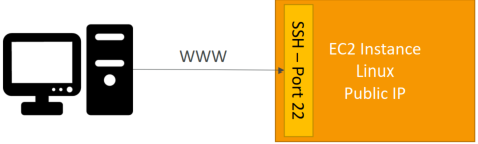
\includegraphics[width=1\linewidth]{images/ssh-connect-to-ec2-instance.png}
	\caption{ssh-connect-to-ec2-instance}
	\label{fig:ssh-connect-to-ec2-instance}
\end{figure}

\subsection{EC2 Instance Connect}

\begin{itemize}
	\item Connect to your EC2 instance within your browser
	\item No need to use your key file that was downloaded
	\item The "magic" is that a temporary key is uploaded onto EC2 by AWS \\ Điều ảo diệu ở đây là AWS tự động tạo một khóa tạm thời lên máy EC2
	\item Works only out-of-the-box with Amazon Linux 2 \\ Hoạt động  ngay lập tức (không cần cấu hình) với Amazon Linux 2
	\item Need to make sure the port 22 is still opened!
\end{itemize}


\subsection{EC2 instances Purchasing Options}

\begin{itemize}
	\item On-Demand Instances : short workload, predictable pricing, pay by second \\  Dành cho khối lượng công việc ngắn, giá cả có thể dự đoán được, và tính phí theo từng giây sử dụng.
	\item Reserved (1 - 3 years)
	\begin{itemize}
		\item Reserved Instance  - long workloads \\  dành cho khối lượng công việc dài hạn
		\item  Convertible Reserved Instance - long workloads with flexible instance  \\ dành cho khối lượng công việc dài hạn nhưng linh hoạt thay đổi loại máy ảo
	\end{itemize}
	\item Saving Plans (1 \& 3 years) - commitment to an amount of usage, long workload \\cam kết sử dụng một mức tài nguyên nhất định, dành cho khối lượng công việc dài hạn
	\item Spot Instance - short workloads, cheap, can lose instance (less reliable) \\ Khối lượng công việc ngắn hạn, rẻ, có thể mất instance (ít tin cậy)
	\item Dedicated Hosts - book an entire physical server, control instance placement \\Đặt trước toàn bộ một máy chủ vật lý và kiểm soát vị trí triển khai của các instance
	\item Dedicate Instances - no other customers will share your hardware
	\item Capacity Reservations - reserve capacity in a specific AZ for any duration \\ Đặt trước dung lượng tài nguyên trong một vùng khả dụng (AZ) cụ thể cho bất kỳ khoảng thời gian nào
	
\end{itemize}


\subsection{EC2 On Demand}

\begin{itemize}
	\item Pay for what you use:
	\begin{itemize}
		\item Linux or Windows - billing per second, after the first minute
		\item All other operating systems - billing per hour
	\end{itemize}
	\item Has the highest cost but upfront payment (Có chi phí cao nhất nhưng không trả tiền trước)
	\item No long-term commitment (Không cần sự cam kết dài hạn)
	\item Recommend for short-term and un-interrupted workloads, where you can't predict how the application will behave \\ Được khuyến nghị cho các khối lượng công việc ngắn hạn và không bị gián đoạn, khi bạn không thể dự đoán được ứng dụng sẽ hoạt động như thế nào
\end{itemize}

\subsection{EC2 Reserved Instances}

\begin{itemize}
	\item Up to 72\% discount compared to On-demand
	\item You reserve a specific instance attributes (Instance Type, Region, Tenancy, OS)
	\item Reservation Period - 1 year (+discount) or 3 years (+++discount)
	\item Payment Options - No Upfront (+), Partial Upfront(+++), All Upfront(+++)
	\item Reserved Instance's Scope - Regional or Zonal (reserve capacity in an AZ)
	\item Recommended for steady-state usage applications (think database) \\ Được khuyến nghị cho các ứng dụng sử dụng ổn định và lâu dài
	\item You can buy and sell in the Reserved Instance Marketplace
	\item Convertible Reserved Instance (Reserved Instance có thể chuyển đổi được)
	\begin{itemize}
		\item Can change the EC2 instance type, instance family, OS, scope and tenancy
	\end{itemize}
\end{itemize} 

\subsection{EC2 Savings Plans}

\begin{itemize}
	\item Get a discount based on long-term usage (up to 72 \% - same as RIs)
	\item Commit to a certain type of usage (Cam kết sử dụng một loại cụ thể)
	\item Usage beyond EC2 Savings Plans is billed at the On-Demand price \\ Phần sử dụng vượt quá gói EC2 Savings Plans sẽ bị tính phí theo giá On-Demand
	\item Locked to a specific instance family \& AWS region
	\item Flexible across (Linh hoạt trên nhiều loại)
	\begin{itemize}
		\item Instance Size 
		\item OS
		\item Tenancy (Host, Dedicated, Default)
	\end{itemize}
\end{itemize}

\subsection{EC2 Spot Instance}

\begin{itemize}
	\item Can get a discount of up to 90\% compared to On-Demand
	\item Instances that you can "lose" at any point of time if your max price is less than the current spot price
	\item The most cost-efficient instances in AWS (Những loại máy ảo tiết kiệm chi phí nhất trong AWS)
	
	\item Useful for workloads that are resilient to failure \\ Hữu ích cho khối lượng công việc chịu lỗi tốt
	\begin{itemize}
		\item Batch jobs
		\item Data analysis
		\item Image processing
		\item Any distributed workloads
		\item Workloads with a flexible start and end time
	\end{itemize}
	\item Not suitable for critical jobs or databases \\ Không phù hợp cho các công việc quan trọng hoặc các cơ sở dữ liệu
\end{itemize}

\subsection{EC2 Dedicated Hosts}

\begin{itemize}
	\item A physical server with EC2 Instance capacity fully dedicated to your use
	\item Allows you address compliance requirements and use your existing server-bound software licenses(per-socker, pre-core, pr-Vm software licenses) \\ Cho phép bạn đáp ứng các yêu cầu tuân thủ và sử dụng các giấy phép phần mềm hiện có vốn ràng buộc với máy chủ
	\item Purchasing Options:
	\begin{itemize}
		\item On-Demand - pay per second for active Dedicate Host
		\item Reserved - 1 or 3 years (No Upfront, Partial Upfront, All Upfront)
	\end{itemize}
	\item The most expensive option
	\item Useful for software that have complicated licensing model (BYOL - Bring Your Own License) \\ Hữu ích cho các phần mềm có mô hình cấp phép phức tạp (BYOL – Mang theo giấy phép của riêng bạn)
	\item Or for companies that have strong regulatory or compliance needs \\ Hoặc dành cho các công ty có nhu cầu tuân thủ pháp lý hoặc quy định nghiêm ngặt
\end{itemize}

\subsection{EC2 Dedicated Instances}

\begin{itemize}
	\item Instances run on hardware that's dedicated to you
	\item May share hardware with other instances in same account (Có thể chia sẻ phần cứng với các instance khác trong cùng tài khoản)
	\item No control over instance placement (can move hardware after stop/start) (Không kiểm soát đối với vị trí đặt instance)
\end{itemize}

\begin{figure}[htbp]
	\centering
	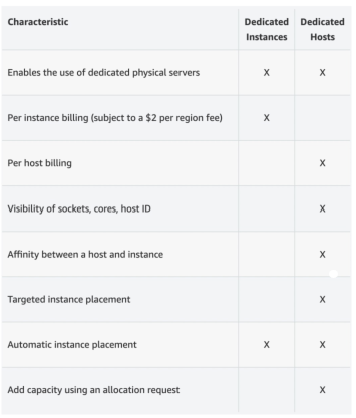
\includegraphics[width=1\linewidth]{images/compare-dedicated-instance-dedicated-hosts.png}
	\caption{compare-dedicated-instance-dedicated-hosts}
	\label{fig:compare-dedicated-instance-dedicated-hosts}
\end{figure}


\subsection{EC2 Capacity Reservations}

\begin{itemize}
	\item Reserve On-Demand instances capacity in a specific AZ for any duration \\ Dữ trữ dung lượng máy chủ On-Demand tại một vùng (AZ) củ thể cho bất kỳ khoảng thời gian nào
	\item You always have access to EC2 capacity when you need it
	\item No time commitment (create/cancel anytime, no billing discounts)
	\item Combine with Regional Reserved Instance and Saving Plans to benefit from billing discounts \\ Kết hợp Regional Reserved Instance và Saving Plans để hưởng lợi từ các khoản giảm giá thanh toán
	\item You're charged at On-Demand rate whether you run instance or not \\ Bạn sẽ bị tính phí theo giá On-Demand dù bạn có có chạy máy ảo hay không
	\item Suitable for short-term, uninterrupted workloads that needs to be in a specific AZ \\ (Phù hợp với các khối lượng công việc ngắn hạn, không bị gián đoạn và cần phải nằm trong một Vùng khả dụng (AZ) cụ thể)
\end{itemize}

\subsection{Which purchasing option is right for me}

\begin{itemize}
	\item On-demand: coming and staying in resort whenever we like, we pay the full price (đến và ở lại resort bất cứ khi nào chúng tôi muốn, trả tiền cho toàn bộ chi phí)
	\item Reserved: like planning ahead and if we plan to stay for a long time, we may be a good discount \\ thích lên kế hoạch cho tương lai và nếu có dự định ở sử dụng trong thời gian dài, chúng ra có thể có giảm giá tốt
	\item Saving Plans: pay a certain amount per hour for certain period and stay in any room type \\ trả một khoản tiền nhất định theo giờ cho khoảng thời gian nhất định và ở trong nhiều loại phòng
	\item Spot instances: the hotel allows people to bid for the empty rooms and the highest bidder keeps the rooms. You can get kicked out at any time \\ Khách sạn cho phép mọi người đấu giá với các phòng trống và người đấu giá cao nhất sẽ giữ phòng. Bạn có thể bị đuổi ra ngoài bất kì thời gian nào
	\item Dedicated Hosts: We book an entire building of the resort
	\item Capacity Reservations: you book a room for a period with full price even you don't stay in it
\end{itemize}

\subsection{AWS charges for IPv4 addresses}

\begin{itemize}
	\item Starting February $1^{st}$ 2024 there's a charge for all Public IPv4 created in your account
	\item \$0.005 per hour of Public IPv4 (~\$3.6) 
	\item For new accounts in AWS, you have a free tier fo the EC2 Service: 750 hours of Public IPv4 per month the first 12 moths
	\item For all other services there is no free tier
	\item What about IPv6?
	\begin{itemize}
		\item Unfortunately, many Internet Service Provide (ISP) around the world don't support IPv6, so the course would not work for some of you \\ Thật không may, nhiều dịch ISP trên thế giới không hỗ trợ IPv6, vì vậy khóa học này không phù hợp với một số bạn
	\end{itemize}
	\item How to troubleshoot charges?
	\begin{itemize}
		\item Go into your AWS Bill
		\item Look into the AWS Public Ip Insight service
		\item Nice article here:
		\url{https://repost.aws/articles/ARknH_OR0cTvqoTfJrVGaB8A/why-am-i-seeing-charges-for-public-ipv4-addresses-when-i-am-under-the-aws-free-tier}
	\end{itemize}
\end{itemize}

\begin{figure}[htbp]
	\centering
	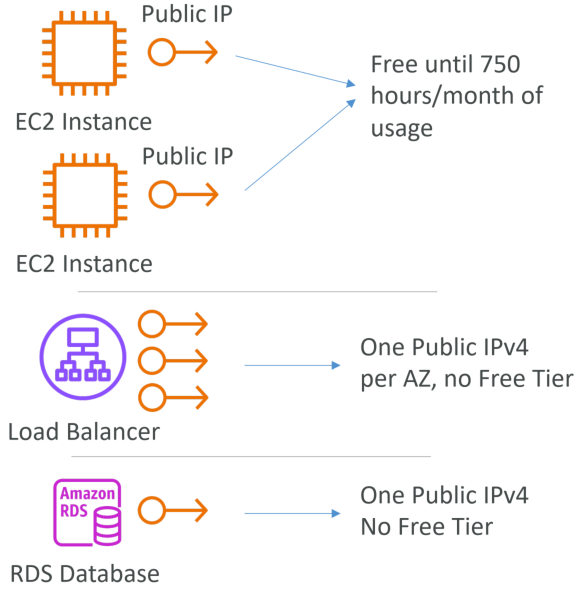
\includegraphics[width=1\linewidth]{images/charge-for-ipv4-addresses.png}
	\caption{charge-for-ipv4-addresses}
	\label{fig:charge-for-ipv4-addresses}
\end{figure}




























































































































